\documentclass[]{report}
\usepackage{graphicx}
\graphicspath{ {resources/images/} }


% Title Page
\title{Utilising peer to peer networking for data transfer over the browser}
\author{Dominic Rathbone}


\begin{document}
\maketitle
\tableofcontents
\


\chapter{Interim planning \& investigation report}
	\section{Project Scope}
		\subsection*{Aims and Objectives}
			The ultimate objective of my project is to investigate the possibility of data transfer over web browsers (in particular audio and video streaming) without the need for a centralised client-server architecture, instead opting for a peer to peer architecture. In order to do so, I will need to research peer to peer networking as well technologies that will allow for it's development in the browser such as WebRTC. In order to test and demonstrate this objective, It will materialize in the form of a web application that people can use to both transfer and stream files (if in a suitable format).
		\subsection*{Stakeholders}
			The stakeholders involved in my project will be myself and the supervisor of my project, Stelios Kapetanakis.
		\subsection*{Methods of Communication}
			Stelios and I have set up a regular meeting once a week on friday at 4pm to review progress and answer any questions. On top of this, we communicate regularly via email and I have set up a private git repository on github to keep my project in which I will give Stelios access to.
		\subsection*{Quality Analysis}
			Success will be measured by the performance of the web application's ability to transfer data. This will be achieved by application metrics recording how fast/reliably files are streamed and transferred under differing amounts of load. Load will be simulated using a load testing tool to mock client connections to the web application.
		
	\section{Specification}
			The first intermediate product will be the signalling server written in Java. This will handle the exchange of client meta data in order to establish the connection between two peers using the web application. I plan to overlap the development of this with the development of the data transfer functionality and user interface of my second deliverable, the web application as manually testing the signalling server will be a lot easier with a partially developed application to test it with.
			
			The first end deliverable will be the client side web application the user interacts with in order to select a file as well as handling sending the meta data to the signalling server and managing the peer to peer data transfer and media streaming. This is broken down into several intermediate products, the data transfer functionality, the media streaming functionality, the many-to-many networking functionality and the user interface. I plan to produce the data transfer functionality first along side the user interface to allow for manual testing. After I have implemented data transfer, I will work on media streaming and forming the peer to peer network topology.
			
			The second end deliverable will be the final report containing documentation and analysis using the metrics	from my application, comparing how it and technologies behind it perform in comparison to others, focusing in particular on how peer to peer over the browser (WebRTC) compares to other methods of data transfer and media streaming.
			
			In terms of risk, I think this will be the largest in my project as it is the only tangible end product and it relies on WebRTC which is a relatively immature technology. As it is new (released in 2011) and it is the only technology at the moment enabling browsers to communicate peer to peer, it has not truly been tried and tested. This means there is a higher potential for problems such as security flaws to exist. Security is a concern with peer to peer networking as issues could allow for unwanted access to your private information. Whilst it would be hard to mitigate risks like this from my position, I think allowing users of the application to enable authentication on the page where the connection lies would give them a level of access control that could avoid unwanted access.
			
	\section{Methodology}
			As a way of tracking the progression of my project, I plan to use Kanban methodology. This is used within software development as a way of incrementally developing applications through iterative cycles. Whilst it is similar to scrum, it doesn't have the stricter framework surrounding it that requires a product owner and scrum master. It also avoids overloading developers with restrictive time-boxed sprints. This methodology is relatively simple and is based around a backlog of tasks from which a developer pulls from in a limited amount, normally 1 or 2 tasks at a time which will are then pushed through the development work flow. In my case, the work flow will be relatively simple:
			\begin{enumerate}
				\item Development iteration per task
				\begin{itemize}
					\item Coding
					\item Code Review: Code will be reviewed by self-evaluation, static code analysis and reviews from other peers and StackExchange.
					\item Manual Testing: If applicable, black box testing will be used to evaluate the code from a user's perspective.
				\end{itemize}
				\item Stakeholder Approval/User Acceptance Testing: Once all the tasks producing a working feature have been completed, it will be tested. 
			\end{enumerate}
		During the coding period of the work flow, I will use a test driven development (TDD) process in which tests are written first and then code is wrote to make the test work. However, I will be fairly lenient with this, only using this process on parts of the code that require stringent testing as writing unnecessary tests will take up development time. 
		\begin{center}
			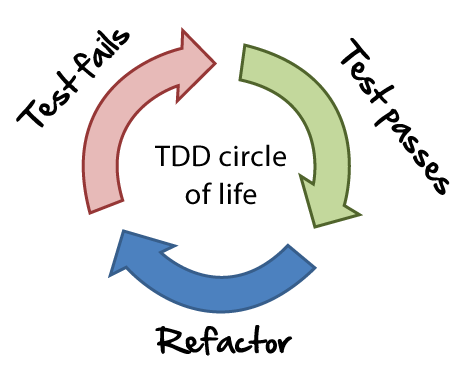
\includegraphics[scale=0.5]{tdd-circle-of-life.png}
		\end{center}

	\section{Literature Review}
		\subsection*{Problems I am trying to solve}
		\subsection*{WebRTC}
		WebRTC is an emerging web technology that enables browsers to communicate real time via a peer to peer connecton, avoiding the need for a centralized server to transfer data between them. This was first released by Google as an open source project to implement real-time communication in the browser in May 2011 \cite{Google WebRTC Release}. It was later drafted as an API definition by W3C which is still a work in progress. \cite{W3C WebRTC Definition}.
		\subsection*{Peer to peer networking topology}
		The entire idea behind my application is based on this peer to peer connection between two browsers. Whilst this one-to-one connection is formed and maintained by WebRTC, it does no more than this. If I want to form an actual many-to-many network of peers then I will have to produce code that will discover and co-ordinate these one-to-one peer connections.
	
		A peer to peer network can be structured in different ways, this structure is referred to as it's topology. There are several different network topologies but I plan to focus on mesh networking as I feel it would best represent the structure that the network of peers using my web application would form. A mesh network is: 
		
		
		\subsection*{Media streaming}
		\subsection*{BackBoneJS framework}
		
	\begin{thebibliography}{9}
		\bibitem{Google WebRTC Release}
		Harald Alvestrand. (2011). Google release of WebRTC source code. Available: http://lists.w3.org/Archives/Public/public-webrtc/2011May/0022.html. Last accessed 29/10/2015.
		\bibitem{W3C WebRTC Definition} 
		Adam Bergkvist, Daniel C. Burnett, Cullen Jennings, Anant Narayanan (until November 2012). (2011). WebRTC 1.0: Real-time Communication Between Browsers. Available: http://www.w3.org/TR/webrtc/. Last accessed 29/10/2015.
		\bibitem{
	\end{thebibliography}

\end{document}          
